La construction des fichiers d'entrée \og grid\fg{} est une étape cruciale pour le bon fonctionnement du modèle CROCO. Ces fichiers définissent la grille spatiale sur laquelle les simulations sont effectuées, et leur précision et leur exactitude sont essentielles pour garantir des résultats fiables. Dans ce chapitre, nous détaillerons les étapes méthodiques que j'ai suivies pour élaborer le script permettant de générer ces fichiers d'entrée. Nous explorerons les défis rencontrés, les solutions adoptées et les optimisations réalisées pour assurer la qualité et l'efficacité de ce processus.

La génération des fichiers \og grid\fg{} est une tâche qui exige une compréhension approfondie non seulement de leur contenu et de leur structure, mais aussi du processus sous-jacent de création. Pour faciliter cette tâche, CROCO met à disposition un ensemble d'outils, dont le CROCO\-Tool, accessible via \url{https://gitlab.inria.fr/croco-ocean/croco\_tools/}. Ce dernier est conçu pour fonctionner avec le logiciel MATLAB. Toutefois, ma familiarité limitée avec MATLAB a rendu l'utilisation de cet outil, et en particulier du module \og make\_grid\fg{} (\url{https://gitlab.inria.fr/croco-ocean/croco\_tools/-/blob/master/Preprocessing\_tools/make\_grid.m}), assez complexe. Bien que la documentation officielle offre des directives, j'ai rencontré des défis liés à la complexité du langage et aux subtilités du script.

Dans le but d'extraire un algorithme clair et compréhensible du script \og make\_grid\fg{}, j'ai entrepris une dissection détaillée de chaque segment de code. Cette démarche, réalisée avec l'aide inestimable de mon maître de stage, a abouti à la découverte de l'algorithme sous-jacent, illustré dans la Figure \ref{fig:AlgoGrid}. Cette étape a été cruciale pour parvenir à reproduire le processus de génération des fichiers \og grid\fg{} de manière autonome, tout en l'adaptant à nos besoins spécifiques.

\newpage

\begin{figure}[h]
	\centering
	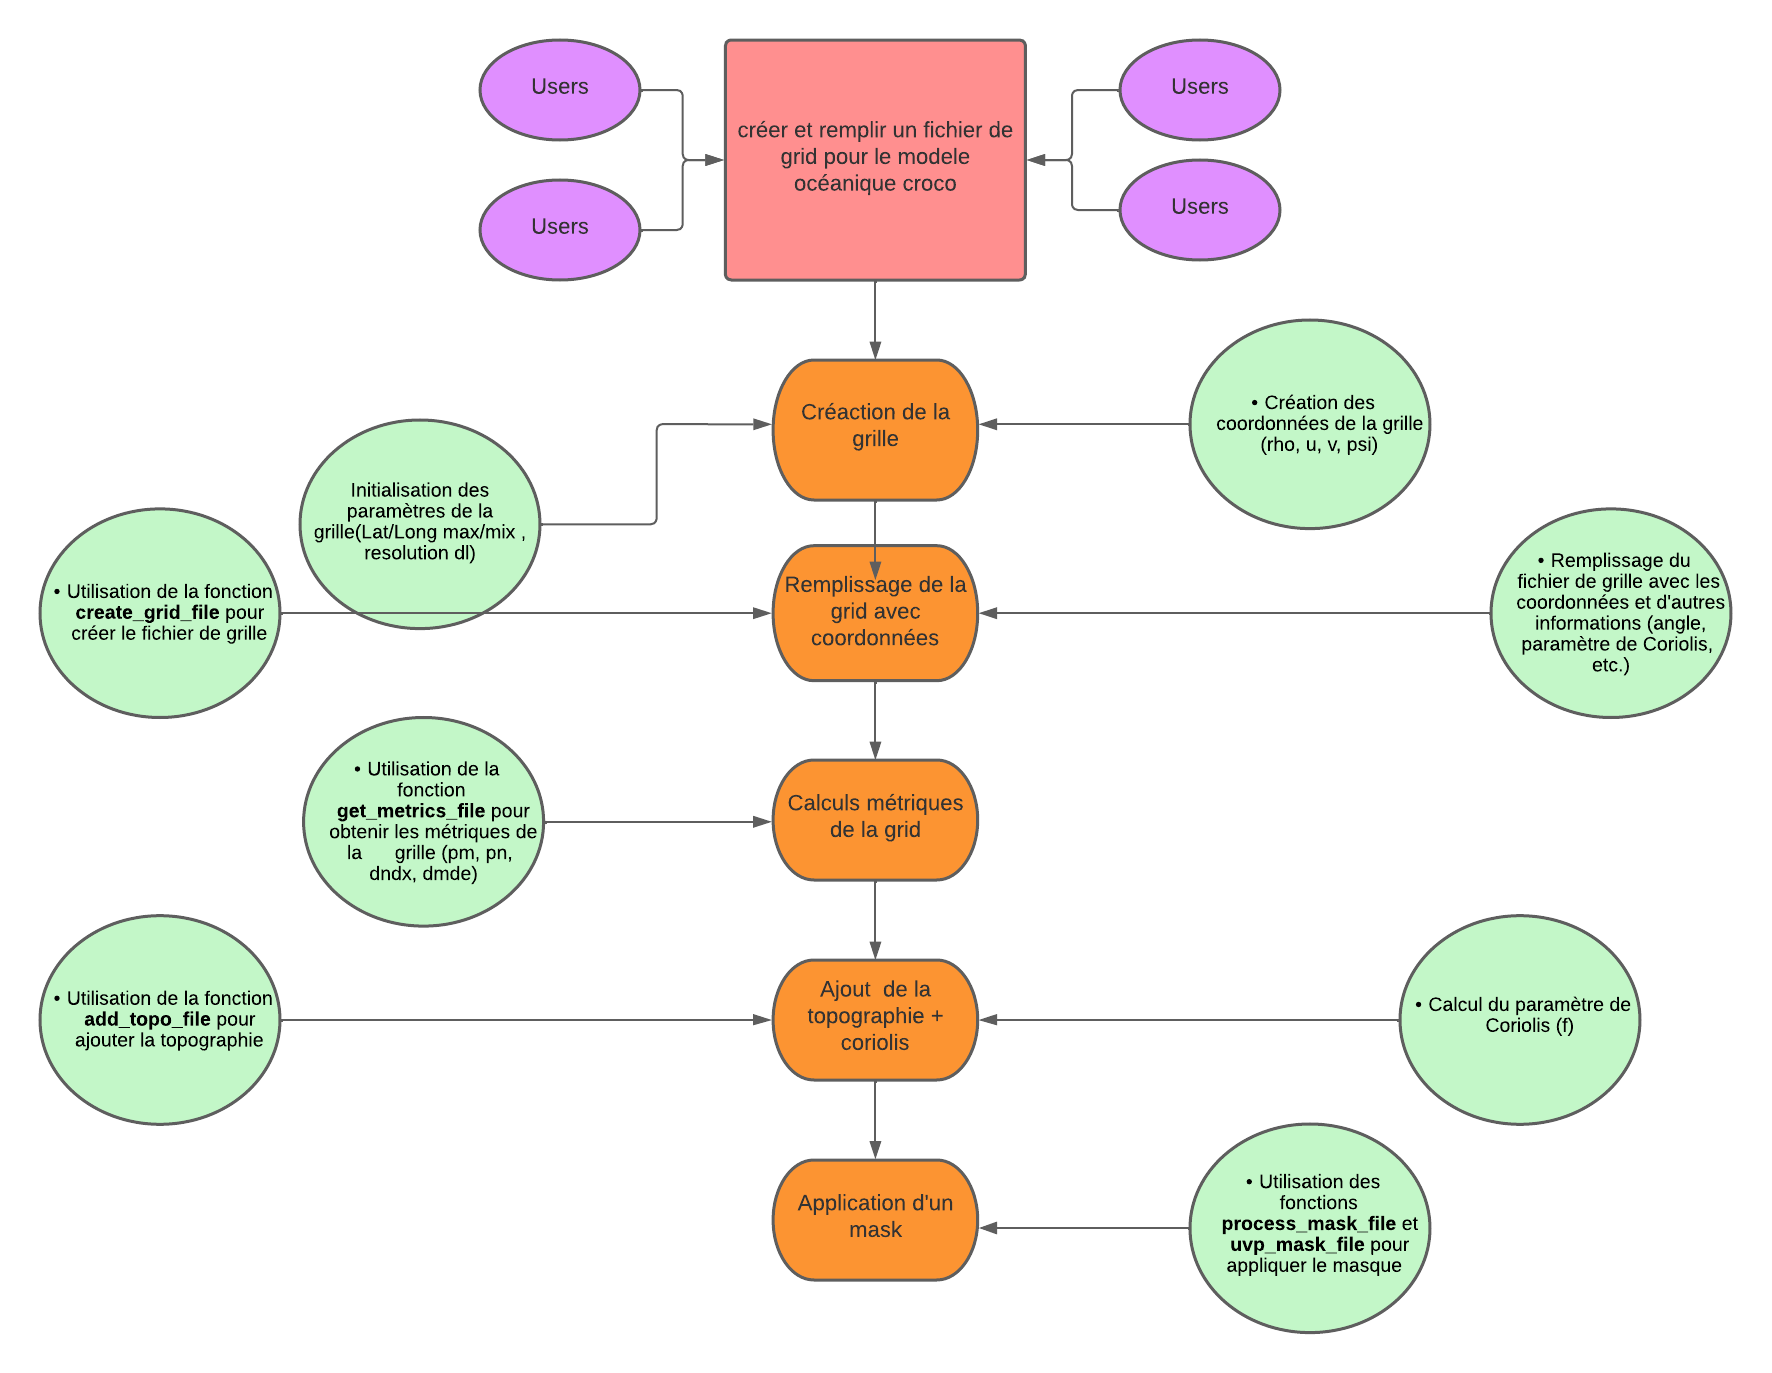
\includegraphics[height=6in]{./IMAGES/DiagrammeGrid.png}
	\caption{Schéma fonctionnel général du script make\_grid.}
	\label{fig:AlgoGrid}
\end{figure}

Suite à cette compréhension approfondie de l'algorithme, l'objectif suivant était clair : adapter ces scripts MATLAB pour les rendre opérationnels dans un contexte différent. En effet, bien que MATLAB soit un outil puissant pour le traitement numérique, notre ambition était de rendre ces scripts plus performants, tout en les intégrant à l'environnement SIG de QGIS. Pour ce faire, la transition vers Python s'est imposée comme une évidence, étant donné sa flexibilité, sa performance et sa compatibilité avec l'API de QGIS. Ainsi, le défi était non seulement de traduire le code, mais aussi d'optimiser et d'adapter les fonctions pour qu'elles s'intègrent harmonieusement dans l'écosystème QGIS, offrant ainsi aux utilisateurs une expérience fluide et intégrée.

Afin d'assurer une compréhension exhaustive du processus de génération des fichiers \og grid\fg{}, il est impératif de décomposer et d'analyser chaque composant de l'algorithme initial. Dans cette section, nous nous attarderons sur les détails techniques de chaque étape de l'algorithme. Nous discuterons également des adaptations nécessaires pour garantir une intégration optimale au sein du plugin QCrocoFlow, tout en respectant les spécificités de l'environnement QGIS. Cette démarche méthodique vise à mettre en lumière les mécanismes fondamentaux, ainsi que les améliorations apportées pour assurer une performance optimale et une compatibilité avec les systèmes d'information géographique (SIG). La suite de ce chapitre se consacrera à une exploration rigoureuse des étapes de transformation et d'adaptation des fichiers \og grid\fg{}.

\subsubsection{Traitement des Données Utilisateur pour la Création du Fichier Grid}

La première étape cruciale dans la création du fichier \textit{grid} a été de définir précisément les entrées nécessaires de la part de l'utilisateur. Ces entrées constituent les informations brutes indispensables pour le bon fonctionnement du script. Plus concrètement, l'utilisateur doit fournir :

\begin{itemize}
	\item Un \textbf{répertoire de travail} : Il s'agit de l'emplacement où les fichiers générés seront sauvegardés et où l'utilisateur pourra les retrouver ultérieurement.
	\item Un \textbf{nom de projet} : Pour identifier et organiser ses simulations.
	\item Un \textbf{titre} : Pour une description plus détaillée de la simulation.
	\item Une \textbf{période de simulation} : L'utilisateur doit spécifier une date de début et une date de fin pour délimiter la durée de sa simulation.
	\item Un \textbf{fichier de topographie} : L'utilisateur a la flexibilité de travailler avec divers formats de fichiers, tels que NetCDF, GRD\footnote{Gradient} ou même TIF\footnote{Tagged Image File Format}.
	\item Une \textbf{résolution} : Elle détermine la taille de chaque maille du fichier grid.
\end{itemize}

Ces informations fournies par l'utilisateur sont essentielles pour adapter le script à des besoins spécifiques et garantir une génération de fichier \textit{grid} conforme aux attentes.

\begin{figure}[h]
	\centering
	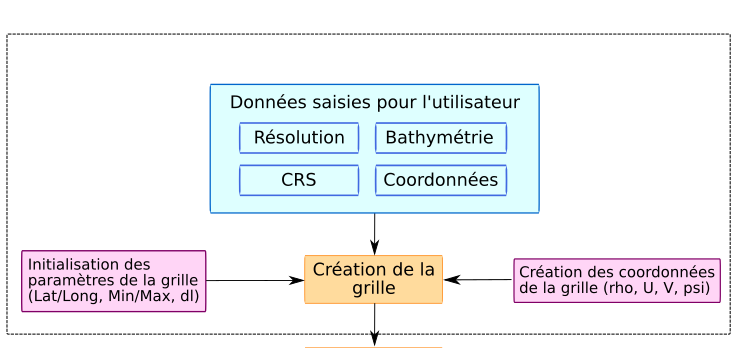
\includegraphics[height=2in]{./IMAGES/figure14.png}
	\caption{Schéma du Processus d'Entrée Utilisateur pour la Génération du Fichier Grid}
	\label{fig:AlgoGrid}
\end{figure}

La Figure~\ref{fig:AlgoGrid} met en évidence l'importance cruciale des choix de l'utilisateur dans l'ensemble du processus. Dans cette optique, la mise en place d'une interface graphique claire et intuitive était primordiale. Elle devait permettre à l'utilisateur de suivre un parcours logique pour renseigner les paramètres essentiels sans ambiguïté.
Pour répondre à cette exigence, j'ai fait appel à l'outil \textit{Qt5 Designer} de QGIS. Cet instrument m'a offert la possibilité de concevoir une interface sur mesure, adaptée aux spécificités de notre projet. Chaque composant de cette interface a été pensé pour optimiser la saisie des informations, assurant ainsi une interaction fluide et efficace pour l'utilisateur. L'expertise apportée par \textit{Qt5 Designer} a été déterminante pour atteindre cet objectif d'excellence en matière d'expérience utilisateur.

\newpage
\begin{figure}[h]
	\centering
	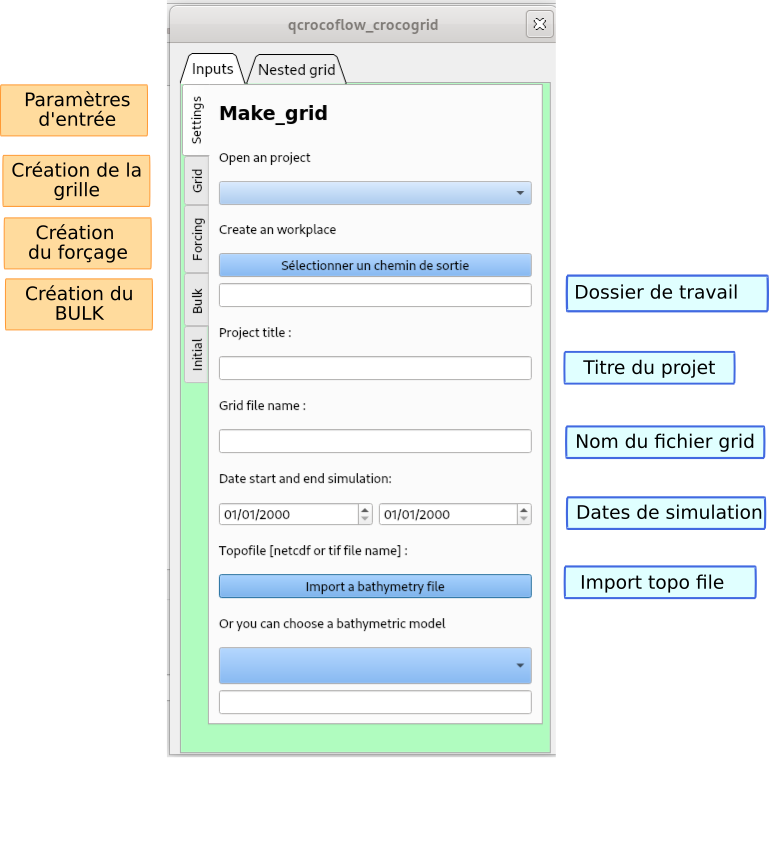
\includegraphics[height=5in]{./IMAGES/paramuser.png}
	\caption{Interface graphique de l'outil Qcrocoflow dans QGIS : Gestion des Paramètres d'Entrée}
	\label{fig:GISUSER}
\end{figure}

Une fois les paramètres saisis, nous exploitons pleinement les capacités offertes par QGIS, en particulier son environnement SIG, pour générer un fichier \og grid\fg{} avec la plus grande précision. Dans un souci de clarté et d'efficacité, j'ai intégré une fonctionnalité lors de la sélection du fichier topographique. Cette fonction permet une visualisation instantanée de son contenu directement sur la carte. De plus, dès l'intégration du fichier dans l'outil, celui-ci est stocké dans une base de données SQL\footnote{Structured Query Language}, intégrée à QGIS. Cela offre à l'utilisateur la commodité de sélectionner directement des fichiers topographiques précédemment chargés dans son projet. Voir la Figure~\ref{fig:BathyF}.

\newpage
\begin{figure}[h]
	\centering
	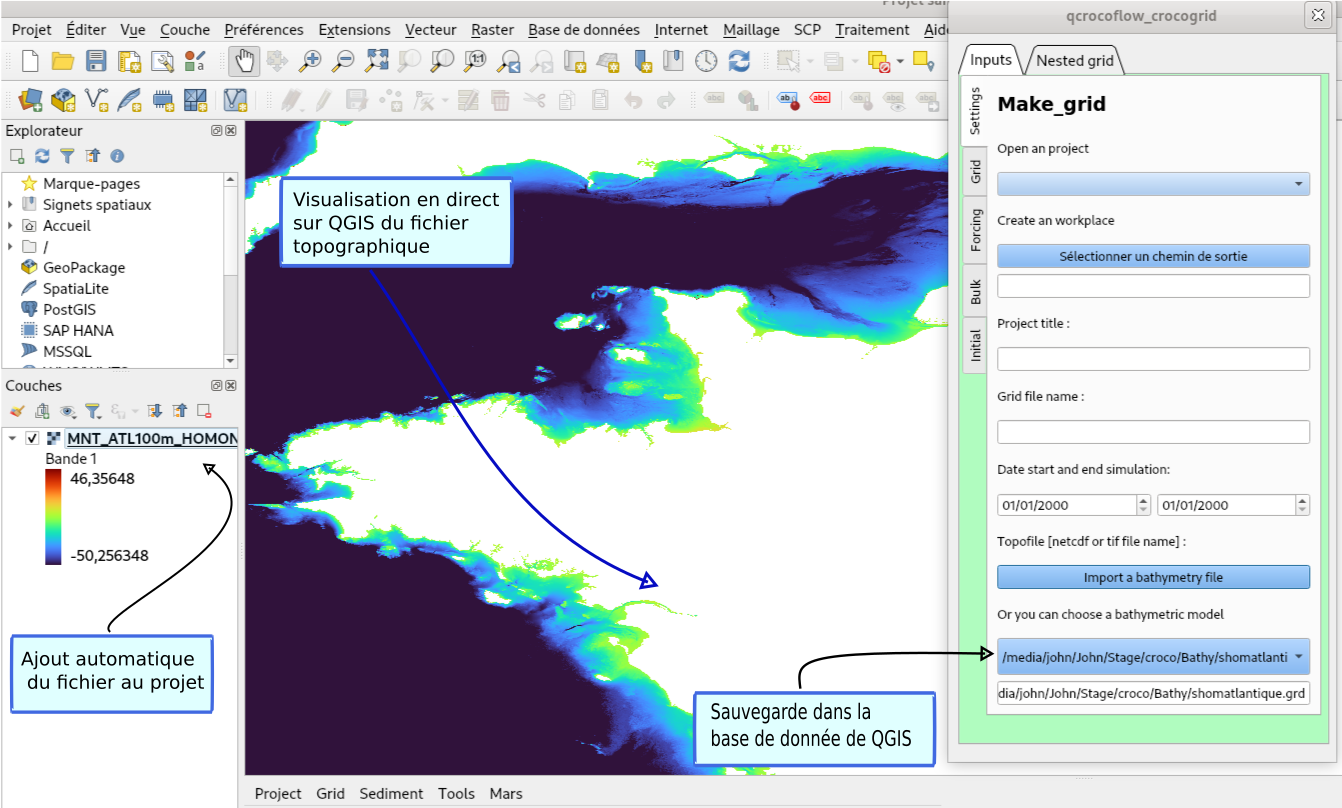
\includegraphics[width=\textwidth]{./IMAGES/BathyF.png}
	\caption{Interface graphique de l'outil Qcrocoflow : intégration et Visualisation d'un Fichier Topographique dans QGIS}
	\label{fig:BathyF}
\end{figure}

Lorsque l'on travaille au sein d'un Système d'Information Géographique (SIG), la gestion des systèmes de référence spatiale est cruciale. Ces systèmes, également connus sous le nom de CRS (pour Coordinate Reference System\footnote{Coordinate Reference System (CRS) : Un système qui utilise des coordonnées pour localiser précisément des points sur la Terre.}), déterminent comment les données sont projetées sur la Terre. Pour le modèle CROCO, le système de référence requis est le WGS84\footnote{WGS84 (World Geodetic System 1984) est la norme mondiale pour l'astronomie, la cartographie et la navigation. Il établit un cadre fixe pour la Terre, indépendant de la position ou de l'orientation de sa surface.}.

Afin d'assurer une intégrité et une précision maximales, j'ai mis en œuvre l'API de QGIS. Cet outil puissant permet de détecter automatiquement le CRS associé à un fichier topographique lors de son importation. QGIS est conçu pour gérer simultanément plusieurs CRS, permettant par exemple d'afficher une carte du monde en WGS84 à côté d'un fichier topographique en Lambert\footnote{Lambert : Un système de projection conique conforme, couramment utilisé pour les cartes de régions étendues, notamment en Europe.}. Si le CRS d'un fichier n'est pas spécifié ou est indétectable, j'ai développé une fonction qui convertit automatiquement ce fichier en WGS84. Cette démarche garantit que toutes les données traitées sont cohérentes et précises, évitant ainsi d'éventuels problèmes lors des étapes ultérieures du processus.~\ref{fig:Gestioncrs}.

\newpage
\begin{figure}[h]
	\centering
	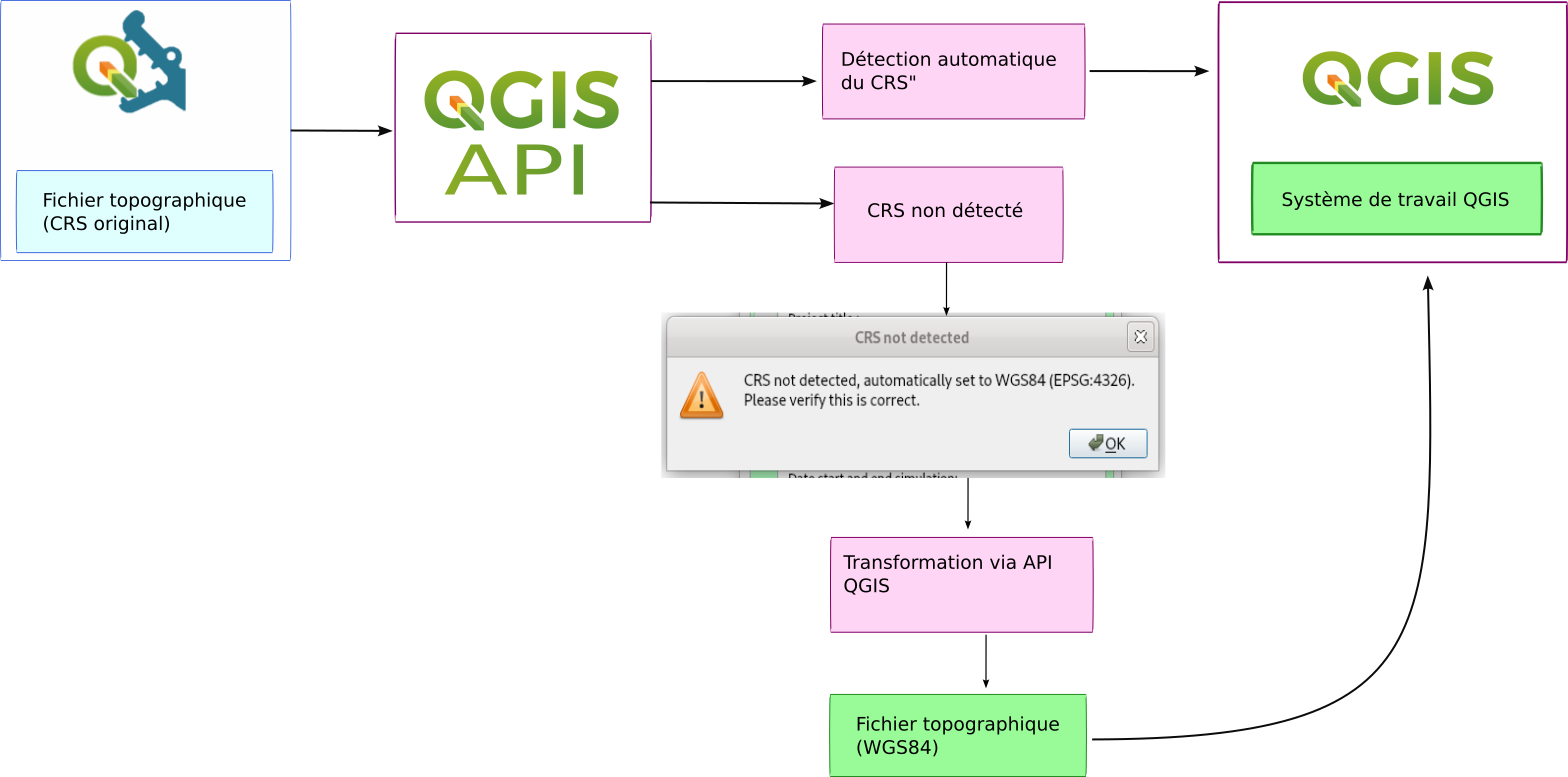
\includegraphics[width=\textwidth]{./IMAGES/Gestioncrs.png}
	\caption{Processus de gestion des CRS dans QGIS pour la création de fichiers \og grid\fg{}}
	\label{fig:BathyF}
\end{figure}